\subsection{Эксперименты и наблюдения(параметры)}

\subsubsection{СС(G) тест}

Для начала убедимся в утверждении выдвинутым ранее: Что $CC(G) \rightarrow 0$ при $n \rightarrow \infty$ в случайном графе:
Взглянем на график случайного графа по модели Erdős–Rényi со средней степенью вершины 5,
с увеличивающейся выборкой:


\begin{figure}[H]
    \centering
    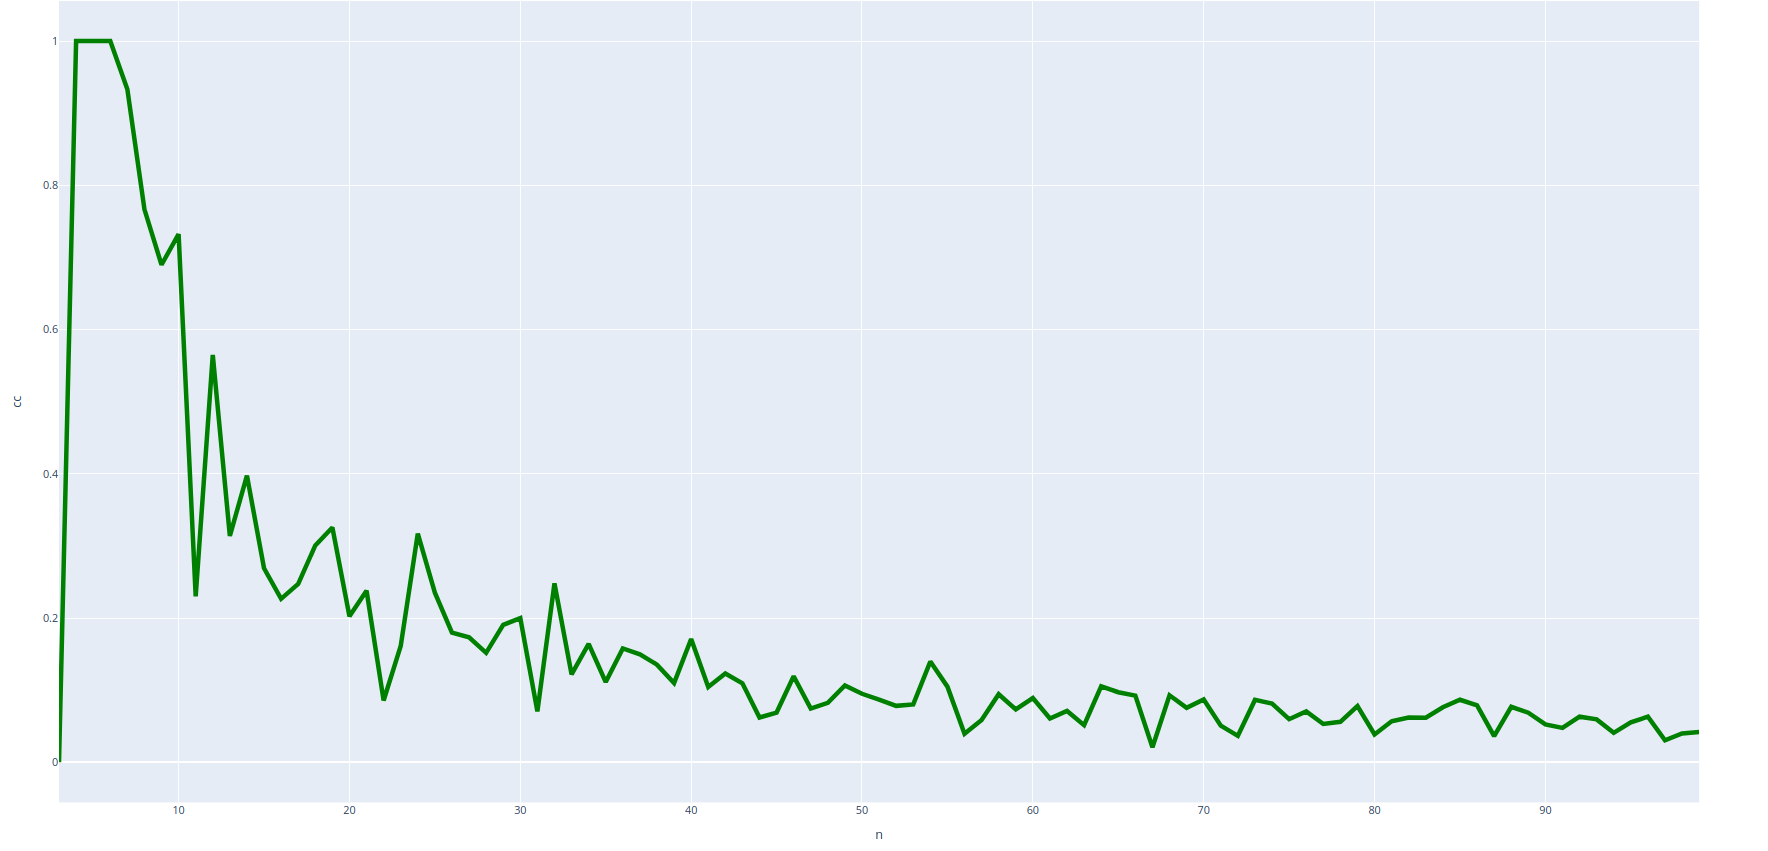
\includegraphics[scale=0.25]{./pictures/random_cc_long_period.png}
    \caption{Зависимость СС(RandomGraph) с ростом выборки} \label{сс от степени вершин}
\end{figure}
Можем наблюдать стабильный нисходящий тренд.

Теперь рассмотрим зависимость коэффицента класстеризации от степени вершин.
В данном примере моя модель содержит 3000 вершин, координаты каждой генерируются случайно 
в диапазона от 0 до 200. Чтобы сравнение было корректным, мне пришлось подобрать параметры
каждого графа так, чтобы степени их вершин примерно совпадали.

\begin{figure}[H]
    \centering
    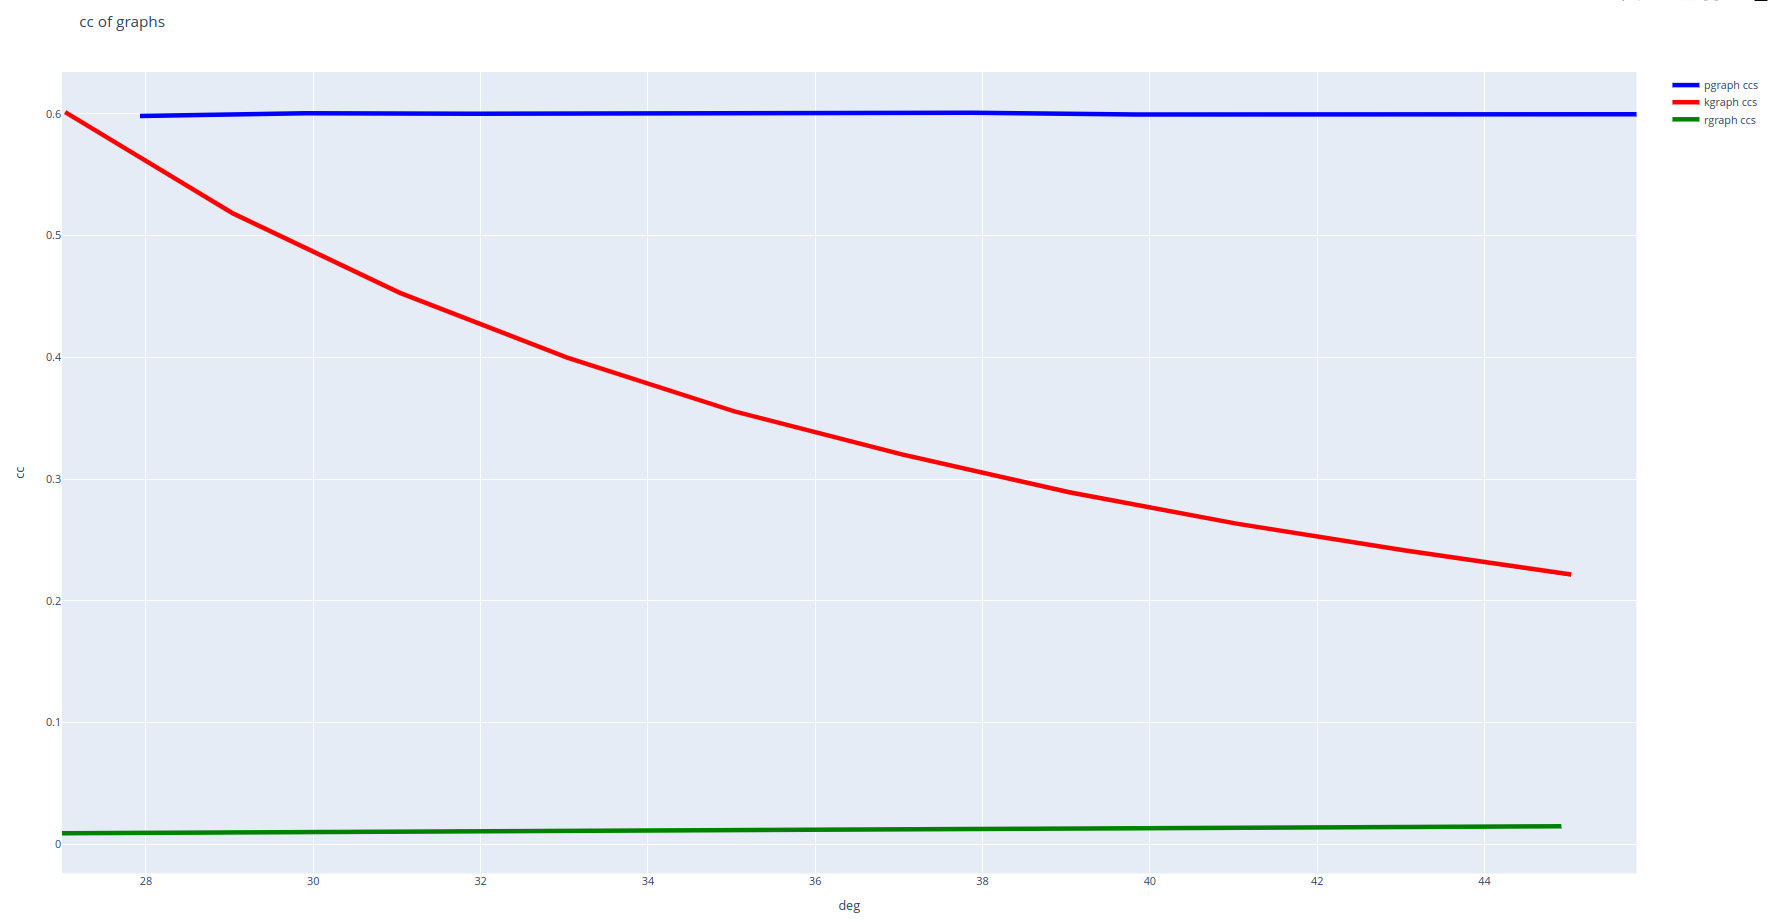
\includegraphics[scale=0.25]{./pictures/cc_better.png}
    \caption{сс от степени вершин} \label{сс}
\end{figure}

Выводы исходя из графика:

\begin{itemize}
    \item граф NNGraph стабильно дуржит коеффицент класстеризации на уровне 0.6 вне
    зависимости от степени вершины 
    \item граф Клайнберга же равне 0.6 только в начале, когда в нём отсутствуют длинные рёбра.
    После чего, по очевидными причинам, с ростом числа случайных рёбер заметен спад.
    \item Случайный граф Erdos-Renye на протяжении всего промежутка имеет неизменный, очень
    слабо класстеризован
\end{itemize}
Результаты согласуются с теоретическими предположениями (Тесные графы имеют не малый коэффицент класстеризации)

Исходные данные:
\begin{itemize}
    \item для графа Клайнберга были выбраны следующие параметры: Кол-во коротких связей: 10. Кол-во длинных
рёбер варьировалось от 0 до 10
    \item для графа NNGraph первым параметром(число повторений) было выбрано 8 (Это оптимальное решение,
обоснование будет чуть дальше). Второй параметр варьировался от 15 до 25
    \item В полностью случайном графе можно явно задать степень вершины, она варьирвалась от 20 до 40
\end{itemize}

\subsubsection{Loss тест}

Теперь измерим одну из самых показательных величин, точность поиска.
Определять точность будем по следующему принципу: Будем запускать алгоритм 1000 раз и 
суммировать расстояние от найденной вершины, до целевой(выбирается случайно).
Чем меньше будет значение, тем лучше наш алгоритм справляется с поиском ближайшего соседа

Взглянем на график(P.s конфигурация графов такая же, как и в прошлом примере):
\begin{figure}[H]
    \centering
    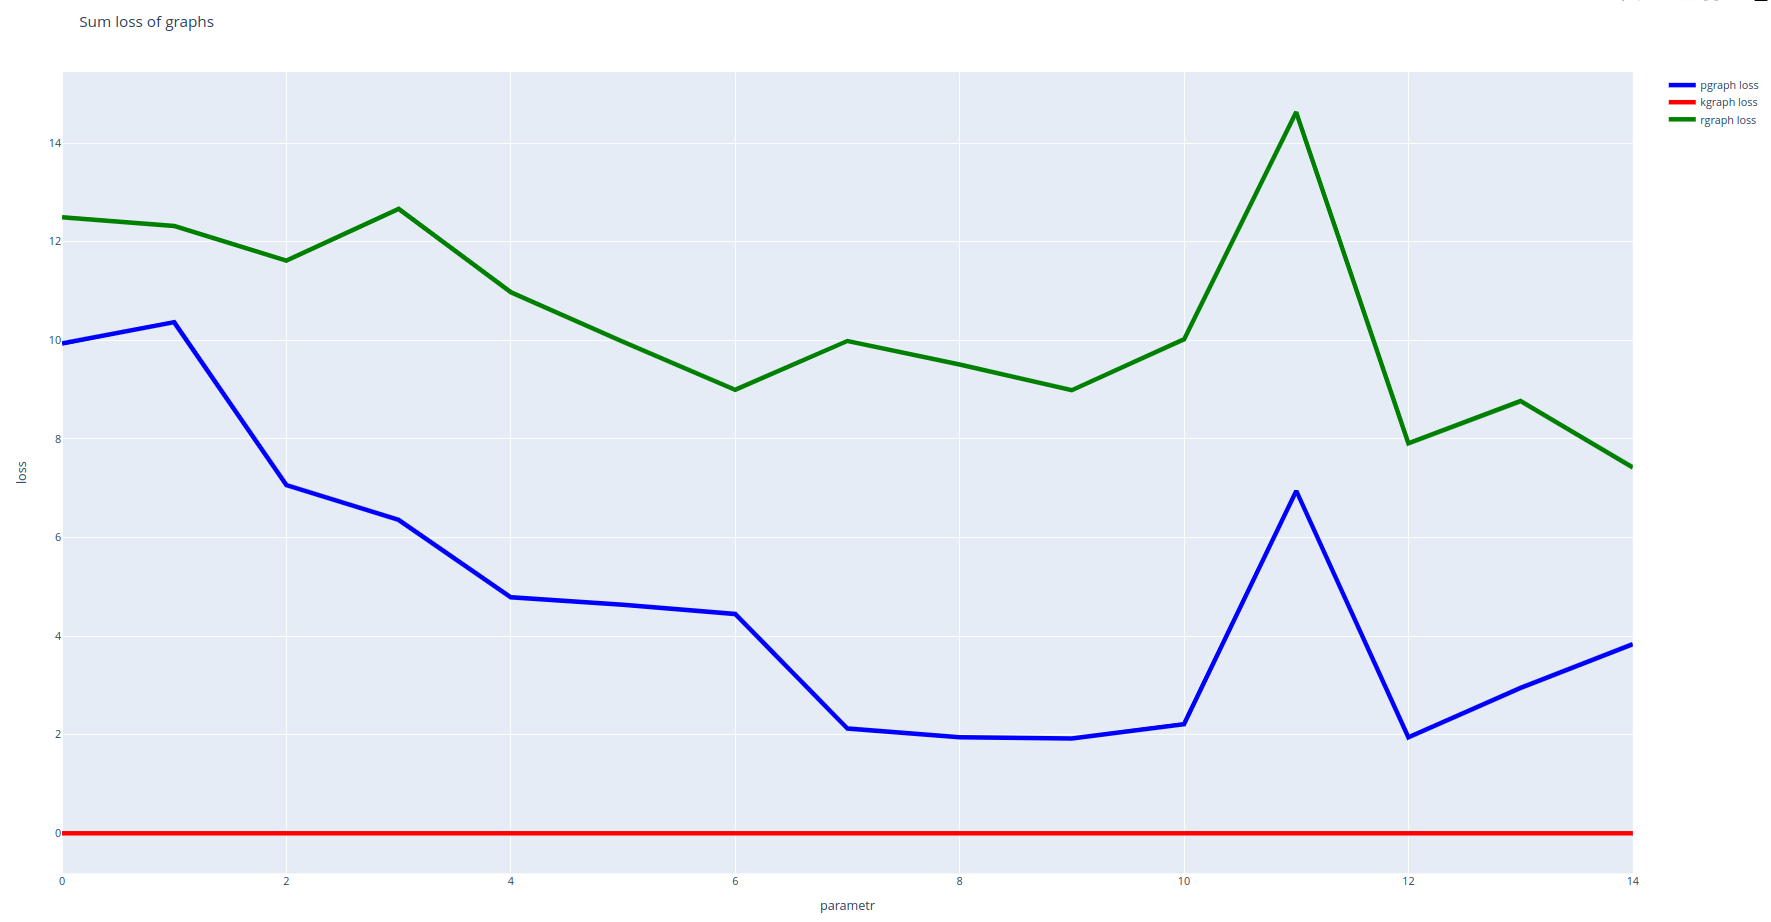
\includegraphics[scale=0.25]{./pictures/sum_loss_imp1.png}
    \caption{Средняя ошибка, параметр "Кол-во повторных поисков" в гарфе NNGraph = 1 } \label{sum_loss}
\end{figure}


Выводы исходя из графика (на данном промежутке):

\begin{itemize}
    \item граф Клайнберга показал себя лучше всех, не допустив ни одной ошибки за все 1000 поисков
    \item граф NNGraph, хоть и работает лучше случайного, но всё ещё стабильно ошибается
\end{itemize}

Теперь рассмотрим только граф NNGraph и увеличим кол-во поисков:
\begin{figure}[H]
    \centering
    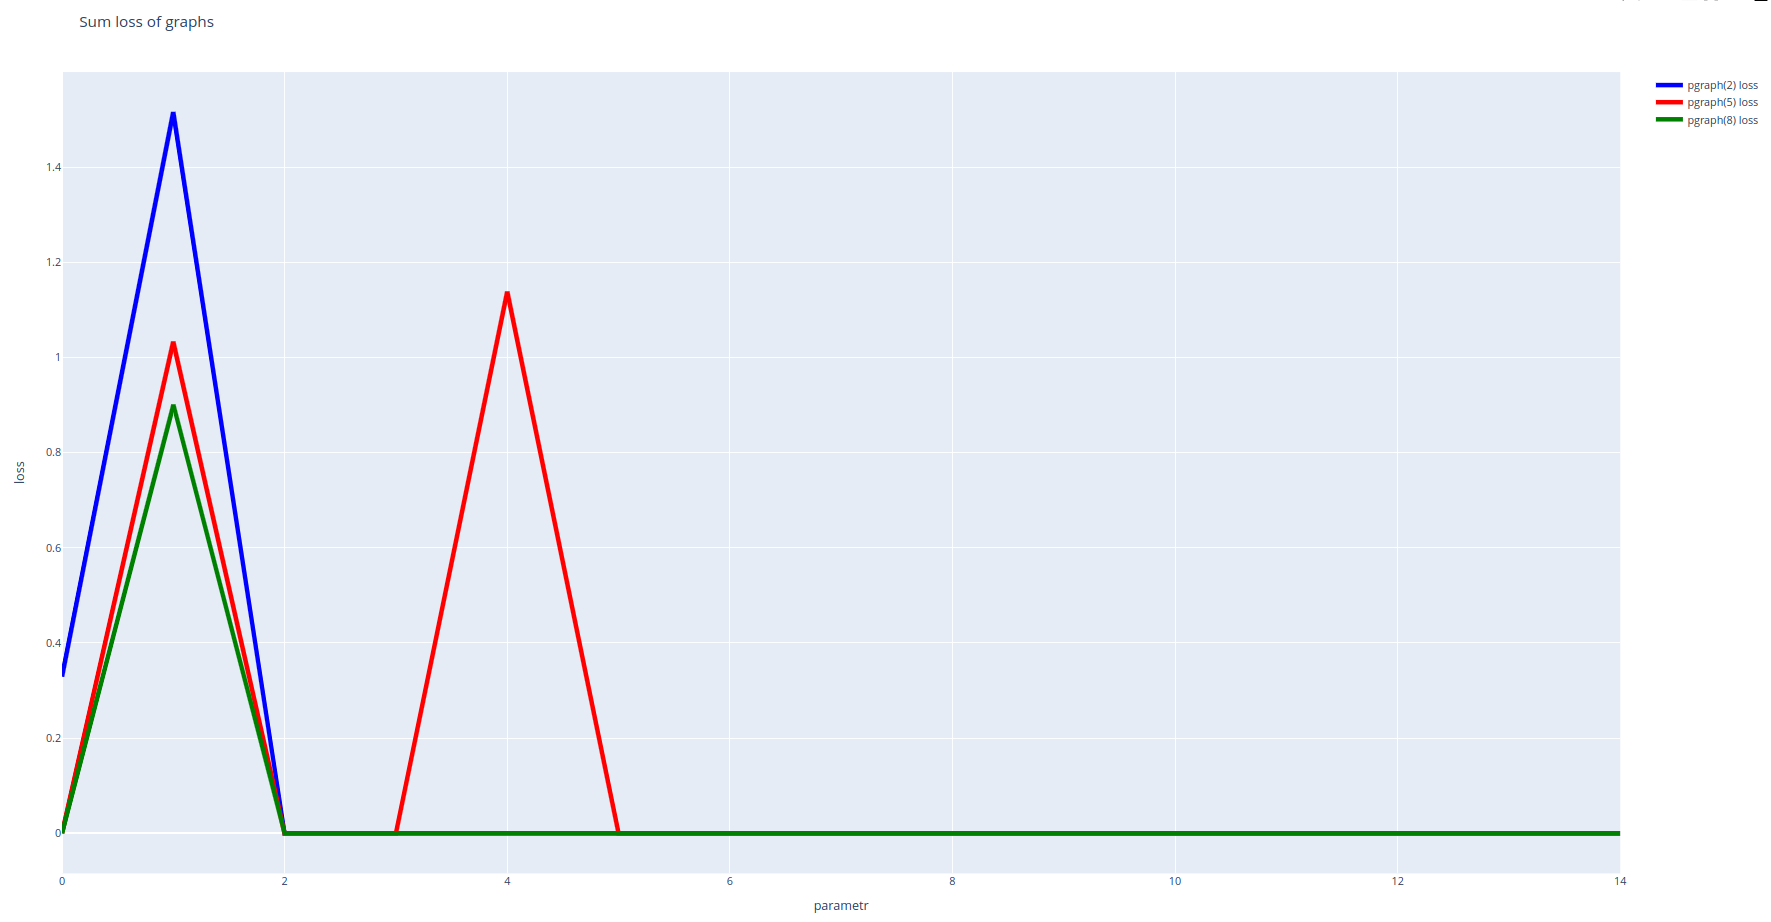
\includegraphics[scale=0.25]{./pictures/sum_loss_Ponomarenko.png}
    \caption{Ошибка при числе поисков 2, 5, 7} \label{sum_loss_Ponomarenko}
\end{figure}

Заметим, что действительно с ростом числа поисков, ошибка по данной метрике становится всё меньше
Из наблюдений Нижегородских математиков достаточное кол-во повторений log(3000) = 8, что согласуется
с наблюдениями

Также поподробнее рассмотрим граф Клайнберга. На этот раз будем варьировать оба его параметра:

\begin{figure}[H]
    \centering
    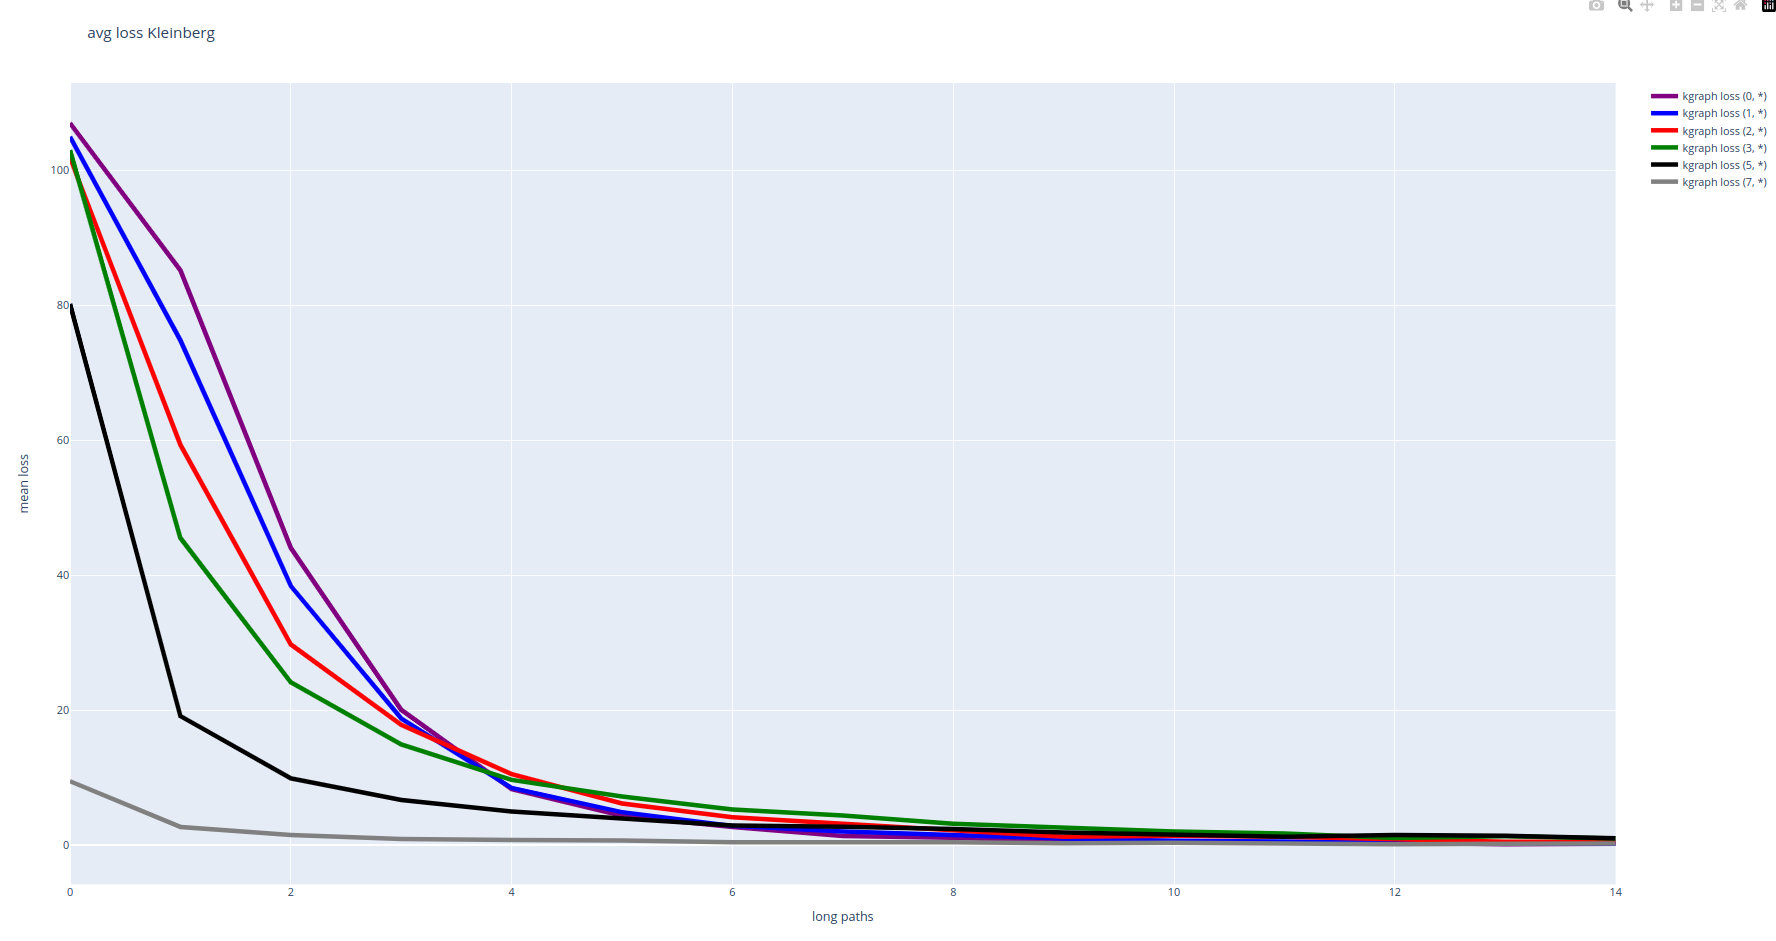
\includegraphics[scale=0.25]{./pictures/Kleinberg_different_parametrs_loss.png}
    \caption{Средняя ошибка в графе Клайнберга при различных параметров} \label{Kleinberg_different_parameters_loss}
\end{figure}

Очевидно, что с увеличением радиуса локальных связей, а также с увеличением кол-ва 
дальних знакомств, loss снижается. Однако здесь нужно обратить внимение именно на скорость
спада. Заметим, что loss графа с меньшим числом локальных связей снижается медленнее
Это также согласуется с предположениями о том, что без локальных связей мы будем часто
попадать в локальные минимумы и копить ошибку

\subsubsection{Тест на среднюю длину пути в жадном поиске}

После измерения ошибки, встаёт логичный вопрос, а сколько шагов требуется жадному алгоритму для
достижения требуемой вершины. 

Начнём с графа Клайнберга, оценим длину пути для параметров с рисунка \ref{Kleinberg_different_parameters_loss}
Рассмотрим 1000 пар случайных вершин графа и усредним полученный путь

\begin{figure}[H]
    \centering
    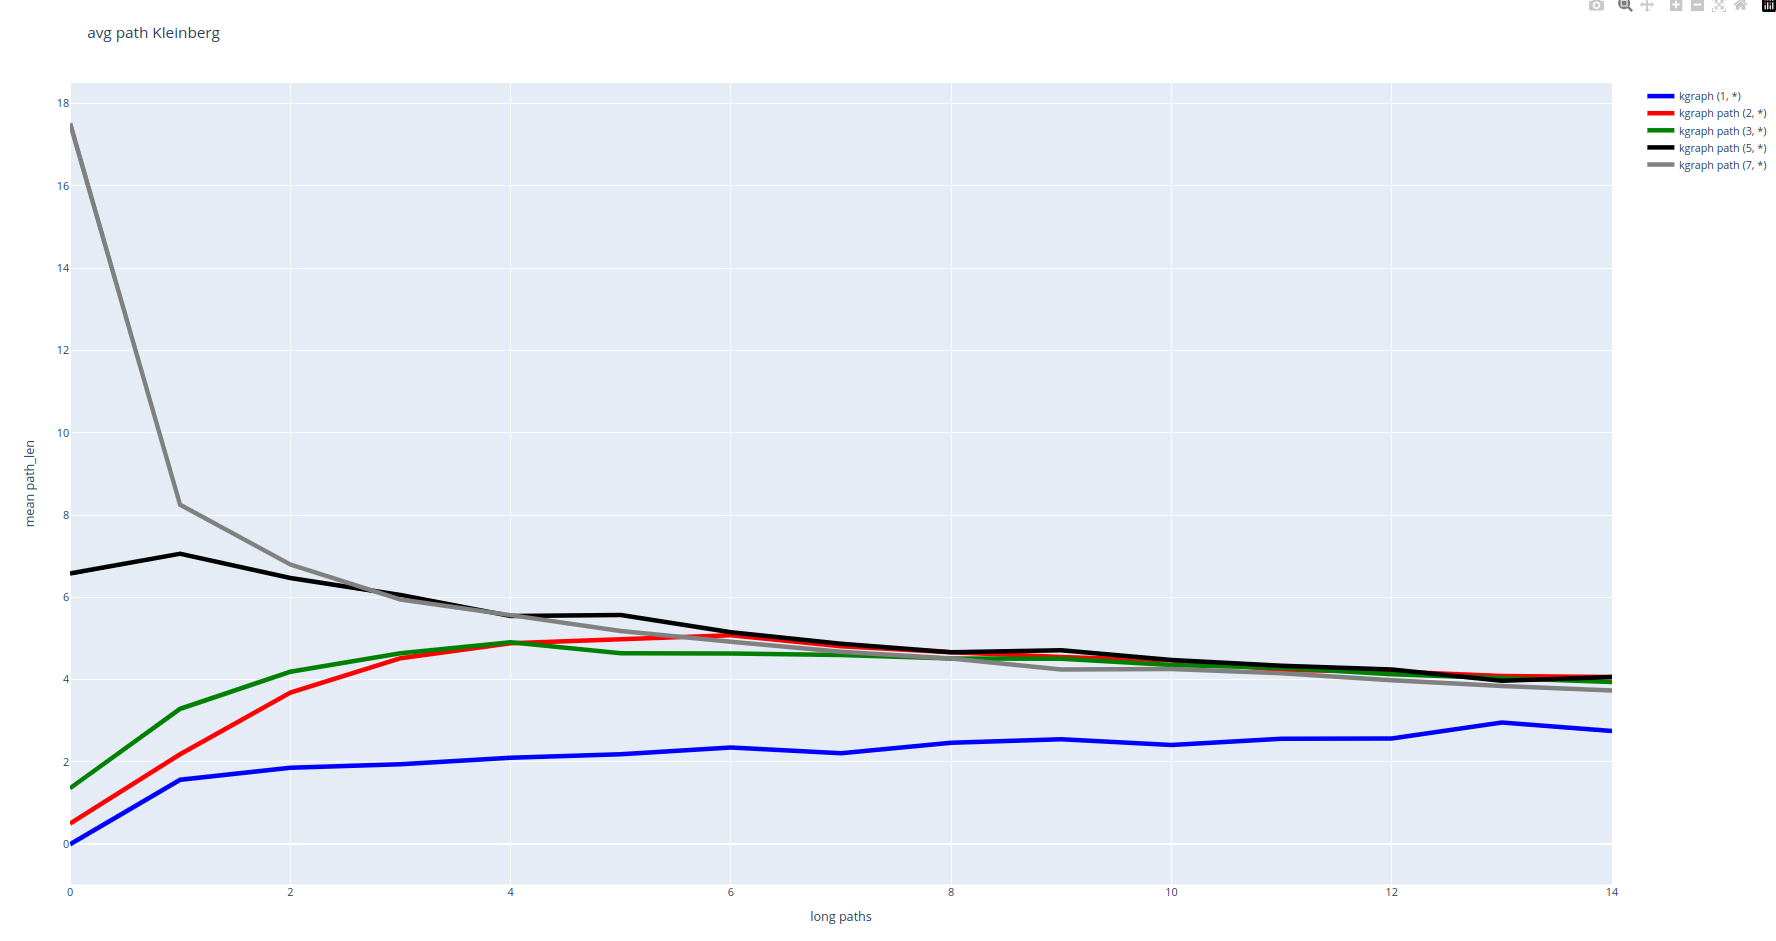
\includegraphics[scale=0.25]{./pictures/Kleinberg_mean_path_len.png}
    \caption{Средняя длиня пути жадного Алгоритма} \label{Kleinberg_different_parameters_path}
\end{figure}

Внимательно изучим график. 
\begin{itemize}
    \item При маленьком радиусе локальных связей, средний путь также мал. Это связано с тем,
что мы быстро упираемся в локальные минимумы и не доходим до истинной вершины. Чтобы это доказать,
достаточно посмотреть на loss при данных параметрах, он велик.

    \item При уменьшении ошибки, наши наблюдения будут всё лучше и лучше оценивать средний диаметр графа
    (Ведь мы просто усредняем длины случайных рёбер (u, v))

    \item рассмотрим набор парамтров, который даёт наименьший loss: (7, *). Заметим, что 
    он хорошо согласуется с теми теоретическими данными, которые мы описывали ранее. В самом начале у нас есть только 
    короткие рёбра, а значит средний путь от одной вершины до другой велик. При увеличении кол-ва длинных связей 
    средний путь начинает резко падать.
    
\end{itemize}